\documentclass[runningheads]{llncs}

\usepackage{graphicx}
\usepackage{amsmath}
\usepackage{amssymb}
\usepackage{booktabs}
\usepackage{algorithm}
\usepackage{algpseudocode}
\usepackage{cite}
\usepackage{url}
\usepackage{lmodern}
\usepackage[T1]{fontenc}
\usepackage{microtype}
\usepackage[hidelinks]{hyperref}

\setlength{\textfloatsep}{2pt plus 1pt minus 1pt}
\setlength{\floatsep}{2pt plus 1pt minus 1pt}
\setlength{\intextsep}{2pt plus 1pt minus 1pt}
\renewcommand{\arraystretch}{0.90}
\renewcommand{\baselinestretch}{0.92}

\newcommand{\doi}[1]{\mbox{\href{https://doi.org/#1}{\texttt{https://doi.org/#1}}}}

\begin{document}
\linespread{0.93}\selectfont

\title{Edge-Assisted Secure Medical Telemetry Using Lightweight Watermarking and Cryptographic Authentication in 5G Healthcare Networks}
\titlerunning{SecureMark-Med: Lightweight Provenance for 5G Medical Networks}

\author{}
\authorrunning{}

\institute{}

\maketitle

\begin{abstract}
Medical images that have already been decrypted at a hospital picture archiving and communication system (PACS) no longer carry the protection of the transport layer. As a result, establishing where an image originated and determining whether it was altered after decryption can become difficult. This work examines SecureMark-Med, an edge-focused verification scheme that combines fragile least-significant-bit (LSB) watermarking with keyed BLAKE3 hashing and ChaCha20-Poly1305 authenticated encryption. Device information, patient indexes, and acquisition timestamps are embedded within the DICOM pixel data. The resulting image is bound to a keyed BLAKE3 integrity token and then protected in transit with ChaCha20-Poly1305. At the receiver, a 30\,s freshness window is also checked to identify delayed or replayed packets. Experiments on a Raspberry Pi 3 Model B+ using clinical CT and radiographic data produced encryption and verification times of 28.61\,ms and 11.92\,ms, respectively; the corresponding AES-256 and HMAC-SHA256 baselines required 84.32\,ms and 31.65\,ms. Image quality remained high after watermark insertion ($\text{PSNR} > 51.4$\,dB and $\text{SSIM} > 0.999$ for the reported 16-bit sets), while localized bit changes were detected by the verification chain.
\keywords{Medical Image Security \and Digital Watermarking \and BLAKE3 \and ChaCha20-Poly1305 \and 5G IoMT \and DICOM Telemetry}
\end{abstract}

\section{Introduction}

Fifth-generation mobile links make it practical for ambulances and mobile triage units to send DICOM scans, including CT, X-ray, and ultrasound images, to a hospital before the patient arrives. This can shorten the time available for clinical preparation, but it also places diagnostic data on a wireless path where interception, modification, or replay is possible. Even a small, unnoticed change in pixel values is undesirable in a clinical image because the interpretation depends on preserving the acquired data.

Conventional transport protection commonly combines a block cipher such as AES-256 with SHA-2-based integrity mechanisms. That approach protects data while it is being transmitted, but three limitations are relevant to an edge-based emergency telemetry setting:
\begin{enumerate}
  \item \textbf{Loss of post-decryption provenance.} After a protected packet is decrypted at the PACS endpoint, the transport wrapper is no longer attached to the plain DICOM object. The image therefore needs an additional mechanism if its source and later integrity are to remain verifiable.
  \item \textbf{Edge computational overhead.} Ambulance gateways may rely on low-power ARM processors without dedicated AES-NI acceleration. On such hardware, conventional cryptographic processing can add latency and increase resource use.
  \item \textbf{Sequential hashing delay.} Large 16-bit images and volumetric data can make sequential hashing a noticeable part of the processing path, particularly when the gateway has limited compute capacity.
\end{enumerate}

SecureMark-Med was designed around these constraints. Rather than relying only on the transport envelope, it places provenance information in the image itself, binds the recovered image to a keyed BLAKE3 token, and uses ChaCha20-Poly1305 for authenticated transport.

\begin{table}[t]
\centering
\caption{Architectural comparison of medical image security schemes.}
\label{tab:comparison}
\small
\begin{tabular}{lccccc}
\hline
Scheme & WM & Encryption & Integrity & Edge-Ready & Freshness Check \\
\hline
Memon and Alzahrani \cite{memon2020prediction} & $\checkmark$ & --- & Partial & --- & --- \\
Anand and Singh \cite{anand2021health}     & $\checkmark$ & --- & ---      & --- & --- \\
Gull et al.\ \cite{gull2021self}         & $\checkmark$ & --- & Local    & --- & --- \\
Singh et al.\ \cite{singh2023robust}        & $\checkmark$ & AES & Checksum & $\checkmark$ & --- \\
\textbf{SecureMark-Med} & \textbf{$\checkmark$} & \textbf{ChaCha20} & \textbf{BLAKE3} & \textbf{$\checkmark$} & \textbf{$\checkmark$} \\
\hline
\end{tabular}
\end{table}

\section{Related Work}

Medical-image watermarking has been studied as a way of keeping ownership, provenance, or integrity information with the image rather than only with the communication channel. Memon and Alzahrani \cite{memon2020prediction} used prediction-error expansion for reversible CT authentication. Anand and Singh \cite{anand2021health} considered multiple watermarking for fused medical images, whereas Alzahrani and Memon \cite{alzahrani2021blind} developed a blind hybrid-domain method aimed at copyright protection. Gull et al.\ \cite{gull2021self} used self-embedding to support tamper detection and localization in smart-health applications.

Work closer to edge deployment has also highlighted the cost of security processing on constrained devices. Singh et al.\ \cite{singh2023robust} studied secure medical-image watermarking in edge-enabled e-healthcare and reported the importance of computational overhead. Tayachi et al.\ \cite{tayachi2023hybrid} proposed a hybrid DICOM watermarking method, while Abirami and Malathy \cite{abirami2024secured} combined chaos-based encryption with a customized deep-learning watermarking model. A broader review by Mahmood et al.\ \cite{mahmood2025secure} discusses remaining issues in secure medical-image sharing and IoMT.

The present design draws on these lines of work but combines the functions in a single edge pipeline. Robust IoMT watermarking \cite{singh2025ensuring}, BLAKE3-based acceleration studies \cite{jasim2025optimizing}, and benchmarking of lightweight cryptography on embedded platforms \cite{buhler2022benchmarking} motivate the choice of primitives. BLAKE3 provides the parallel tree-hash structure used for the keyed integrity token \cite{oconnor2020blake3}, ChaCha20-Poly1305 supplies authenticated encryption \cite{nir2018chacha20}, and the image representation follows the DICOM standard maintained by NEMA \cite{nema2024dicom}.

\section{Proposed SecureMark-Med Framework}

The proposed pipeline performs three linked tasks before transmission: it inserts provenance information into the image, computes a cryptographic integrity token over the watermarked data, and finally applies authenticated encryption. The receiver reverses these steps while checking freshness and consistency at each stage.

\subsection{Watermark Embedding}
Let $I \in \mathbb{R}^{M \times N}$ represent a 16-bit grayscale DICOM image. The watermark payload $W$ combines patient, hospital, device, and acquisition-time information:
\begin{equation}
  W = ID_{pat} \parallel ID_{hosp} \parallel DevID \parallel T_s
\end{equation}
The payload is serialized as $B=\{b_0,\dots,b_{L-1}\}$. Each bit is written into the least significant bit of a successive image pixel:
\begin{equation}
  \tilde{p}(i,j) = \bigl(p(i,j) \land {\sim}1\bigr) \lor b_k, \quad k = i \cdot N + j, \quad \forall\,k < L
\end{equation}
Only the least significant bit is changed, so the absolute modification of an affected pixel is at most one gray-level unit. In this study the watermark is intentionally fragile: a later pixel modification or lossy re-encoding can disturb the embedded sequence and is therefore treated as an integrity warning. This behavior is suitable for the lossless telemetry profile considered here, where preserving the acquired pixel matrix is the priority.

\subsection{Integrity Token and Authenticated Encryption}
After embedding, the watermarked image $I_w$ is serialized as the byte buffer $M_{bytes}$. A keyed BLAKE3 token $\tau$ is then calculated with the shared 256-bit secret $K_{sec}$:
\begin{equation}
  \tau = \text{BLAKE3}_{\text{keyed}}(K_{sec}, DevID \parallel M_{bytes} \parallel T_s)
\end{equation}
The image, token, and timestamp are grouped as $M = (I_w \parallel \tau \parallel T_s)$. This payload is encrypted with ChaCha20-Poly1305 using $K_{enc}$ and a fresh 96-bit CSPRNG nonce $\mathcal{N}$:
\begin{equation}
  (C,\,\text{Tag}) = \text{ChaCha20-Poly1305-Encrypt}(K_{enc},\mathcal{N},M)
\end{equation}
The transmitted datagram is $P = \mathcal{N} \parallel C \parallel \text{Tag}$. The AEAD tag protects the transport packet itself, whereas the keyed BLAKE3 value and embedded watermark provide checks tied to the recovered application data. Keeping these roles separate is useful after decryption, because provenance can still be evaluated at the PACS workstation even though the transport envelope has been removed.

\begin{algorithm}[htbp]
\caption{Receiver Verification and Provenance Extraction}
\label{alg:verification}
\begin{algorithmic}[1]
\Require Datagram $P$; keys $K_{enc}, K_{sec}$; expected metadata $DevID, W_{exp}$; clock $T_{now}$
\Ensure Verdict $\in \{\text{Authentic},\,\text{Tampered},\,\text{Stale}\}$
\State Parse $\mathcal{N} \parallel C \parallel \text{Tag} \gets P$
\State $M \gets \text{ChaCha20-Poly1305-Decrypt}(K_{enc}, \mathcal{N}, C, \text{Tag})$
\If{$M = \bot$} \Return \textbf{Tampered} (AEAD tag failure) \EndIf
\State Deconstruct $(I_w \parallel \tau \parallel T_s) \gets M$
\If{$\vert{}T_{now} - T_s\vert{} > 30\,\text{s}$} \Return \textbf{Stale} (Expired freshness window) \EndIf
\State $\tau_{\mathit{calc}} \gets \text{BLAKE3}_{\text{keyed}}(K_{sec}, DevID \parallel \text{Serialize}(I_w) \parallel T_s)$
\If{$\tau \neq \tau_{\mathit{calc}}$} \Return \textbf{Tampered} (Cryptographic hash mismatch) \EndIf
\State Extract $W_{ext}$ from LSBs of $I_w$
\If{$W_{ext} \neq W_{exp}$} \Return \textbf{Tampered} (Provenance mismatch) \EndIf
\State \Return \textbf{Authentic}
\end{algorithmic}
\end{algorithm}

At reception, the packet is first authenticated and decrypted. A failed AEAD check immediately marks the packet as tampered. A valid packet is then tested against the 30\,s freshness window, followed by recomputation of the keyed BLAKE3 token and extraction of the LSB watermark. The packet is accepted only when all four checks succeed.

\begin{figure}[htbp]
\centering
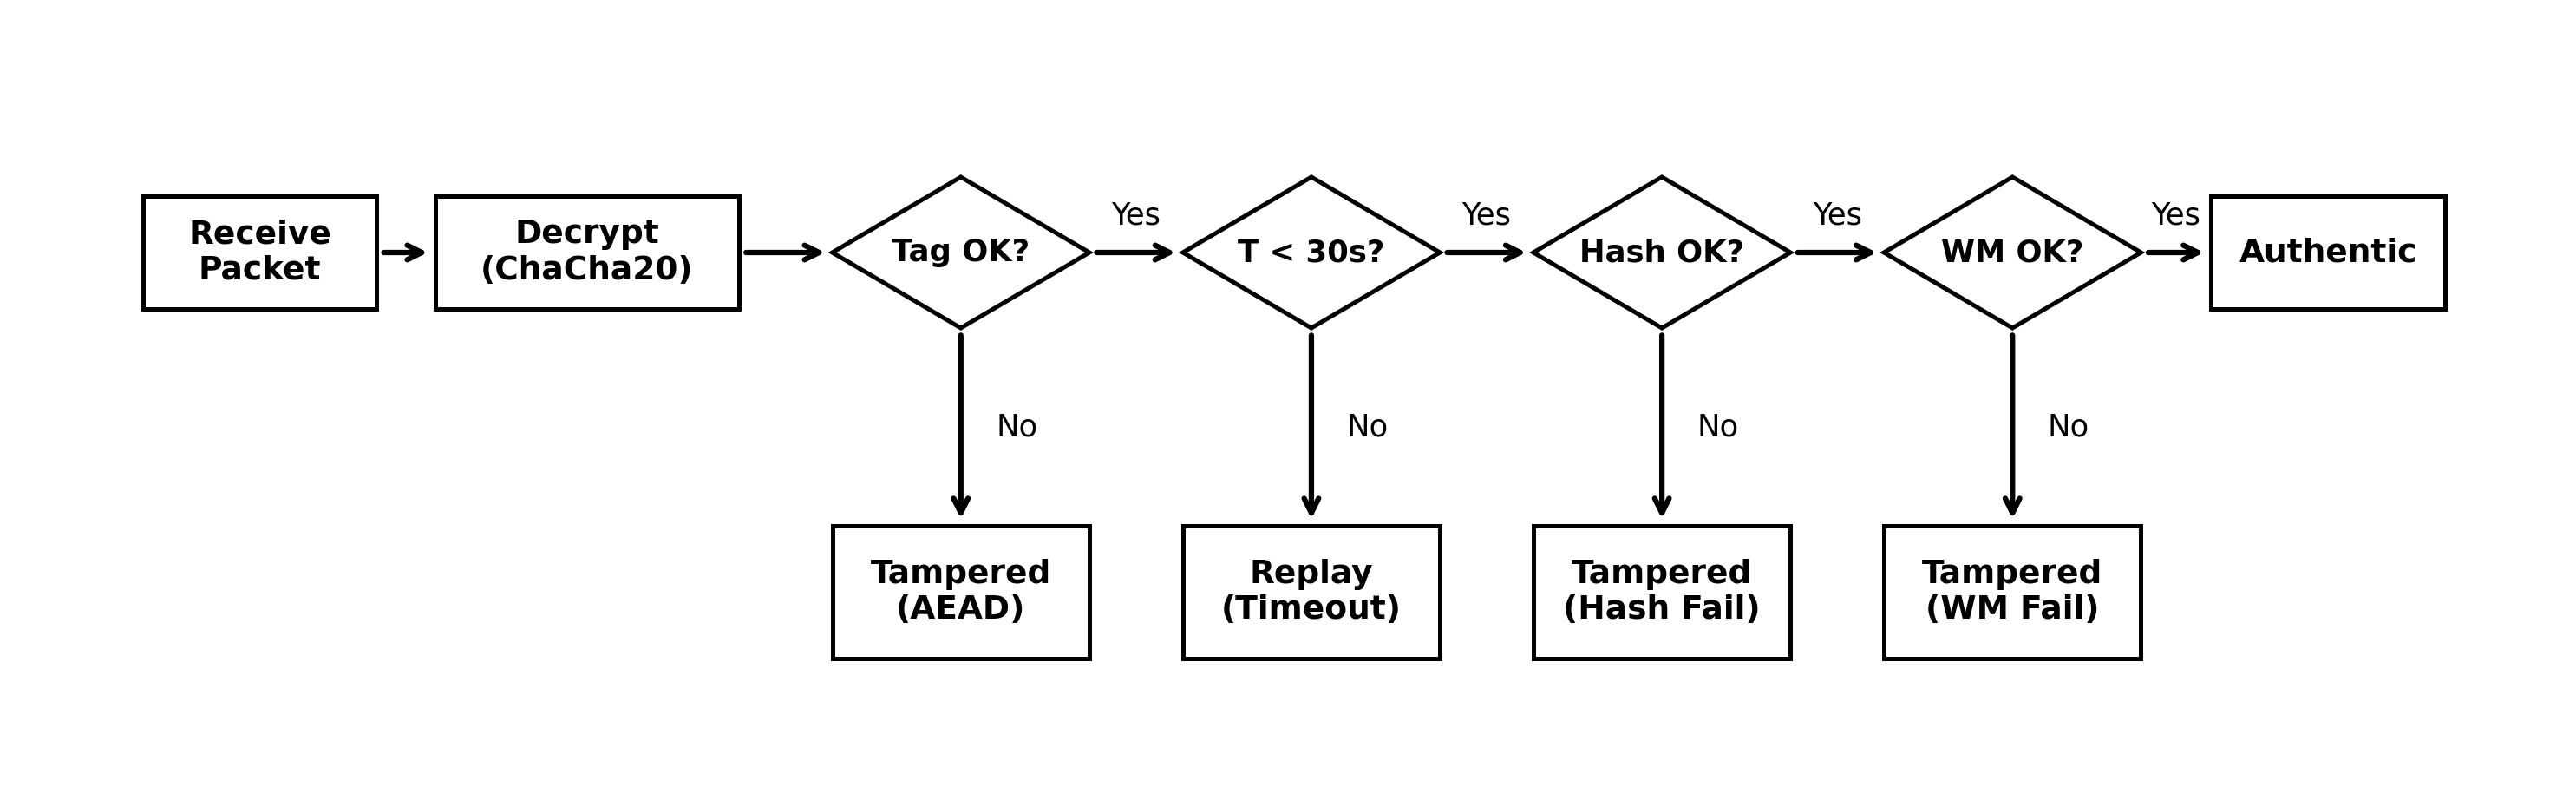
\includegraphics[width=0.95\textwidth]{fig_architecture.png}
\vspace{-5pt}
\caption{Logical architecture and decision flow of the receiver verification stage, showing the sequence of cryptographic, freshness, and provenance checks.}
\label{fig:architecture}
\end{figure}

\section{Experimental Results and Discussion}

\begin{table}[t]
\centering
\caption{Unified Dataset Attributes and Evaluated Diagnostic Fidelity Metrics}
\label{tab:dataset_fidelity}
\small
\begin{tabular}{@{}lcclrrc@{}}
\toprule
Modality & Resolution & Bit Depth & DICOM File Size & PSNR (dB) & SSIM & BER (\%) \\
\midrule
Cranial CT         & $512 \times 512$   & 16-bit & 512\,KB & 51.42 & 0.9997 & 0.00 \\
Chest X-Ray        & $1024 \times 1024$ & 16-bit & 2.0\,MB & 52.14 & 0.9998 & 0.00 \\
Abdominal MRI      & $512 \times 512$   & 16-bit & 512\,KB & 53.08 & 0.9999 & 0.00 \\
Cardiac Ultrasound & $640 \times 480$   & 8-bit  & 900\,KB & 49.82 & 0.9989 & 0.00 \\
\bottomrule
\end{tabular}
\end{table}

The experiments used a Raspberry Pi 3 Model B+ (Broadcom BCM2837B0, four Cortex-A53 cores at 1.4\,GHz, Linux kernel 6.1) as the ambulance-side gateway and an AMD Ryzen workstation at the receiving side. BLAKE3 (v1.5) and chacha20poly1305 (v0.10) were implemented in Rust and exposed to the test environment through \texttt{pyo3} bindings. Each timing result was obtained from 1{,}000 independent trials after 100 warm-up iterations. The reported cryptographic timings exclude network I/O and the spatial watermarking step, so they should be interpreted as local processing costs rather than complete end-to-end system latency.

The DICOM instances listed in Table~\ref{tab:dataset_fidelity} span CT, chest radiography, MRI, and ultrasound. For the reported 16-bit images, PSNR remained above $51.4\,\text{dB}$ and SSIM above 0.999. The ultrasound case, which is 8-bit, produced a PSNR of $49.82\,\text{dB}$ and an SSIM of 0.9989. BER was 0.00\% for every listed modality. These measurements indicate that changing only the LSB produces very small image differences in the tested data.

\subsection{Processing Latency and Resource Consumption}
Figure~\ref{fig:benchmarks} summarizes the processing measurements. ChaCha20-Poly1305 required $28.61\,\text{ms}$ for encryption, compared with $84.32\,\text{ms}$ for AES-256 in the reported test setup. RSA-2048 took $132.47\,\text{ms}$ and is included only as a reference for asymmetric key-encapsulation cost rather than as an alternative bulk-image cipher. For integrity processing, the keyed BLAKE3 stage required $11.92\,\text{ms}$, whereas HMAC-SHA256 required $31.65\,\text{ms}$. Peak memory use was $70.16\,\text{MB}$ for the proposed implementation and $198.45\,\text{MB}$ for the baseline implementation.

\begin{figure}[htbp]
\centering
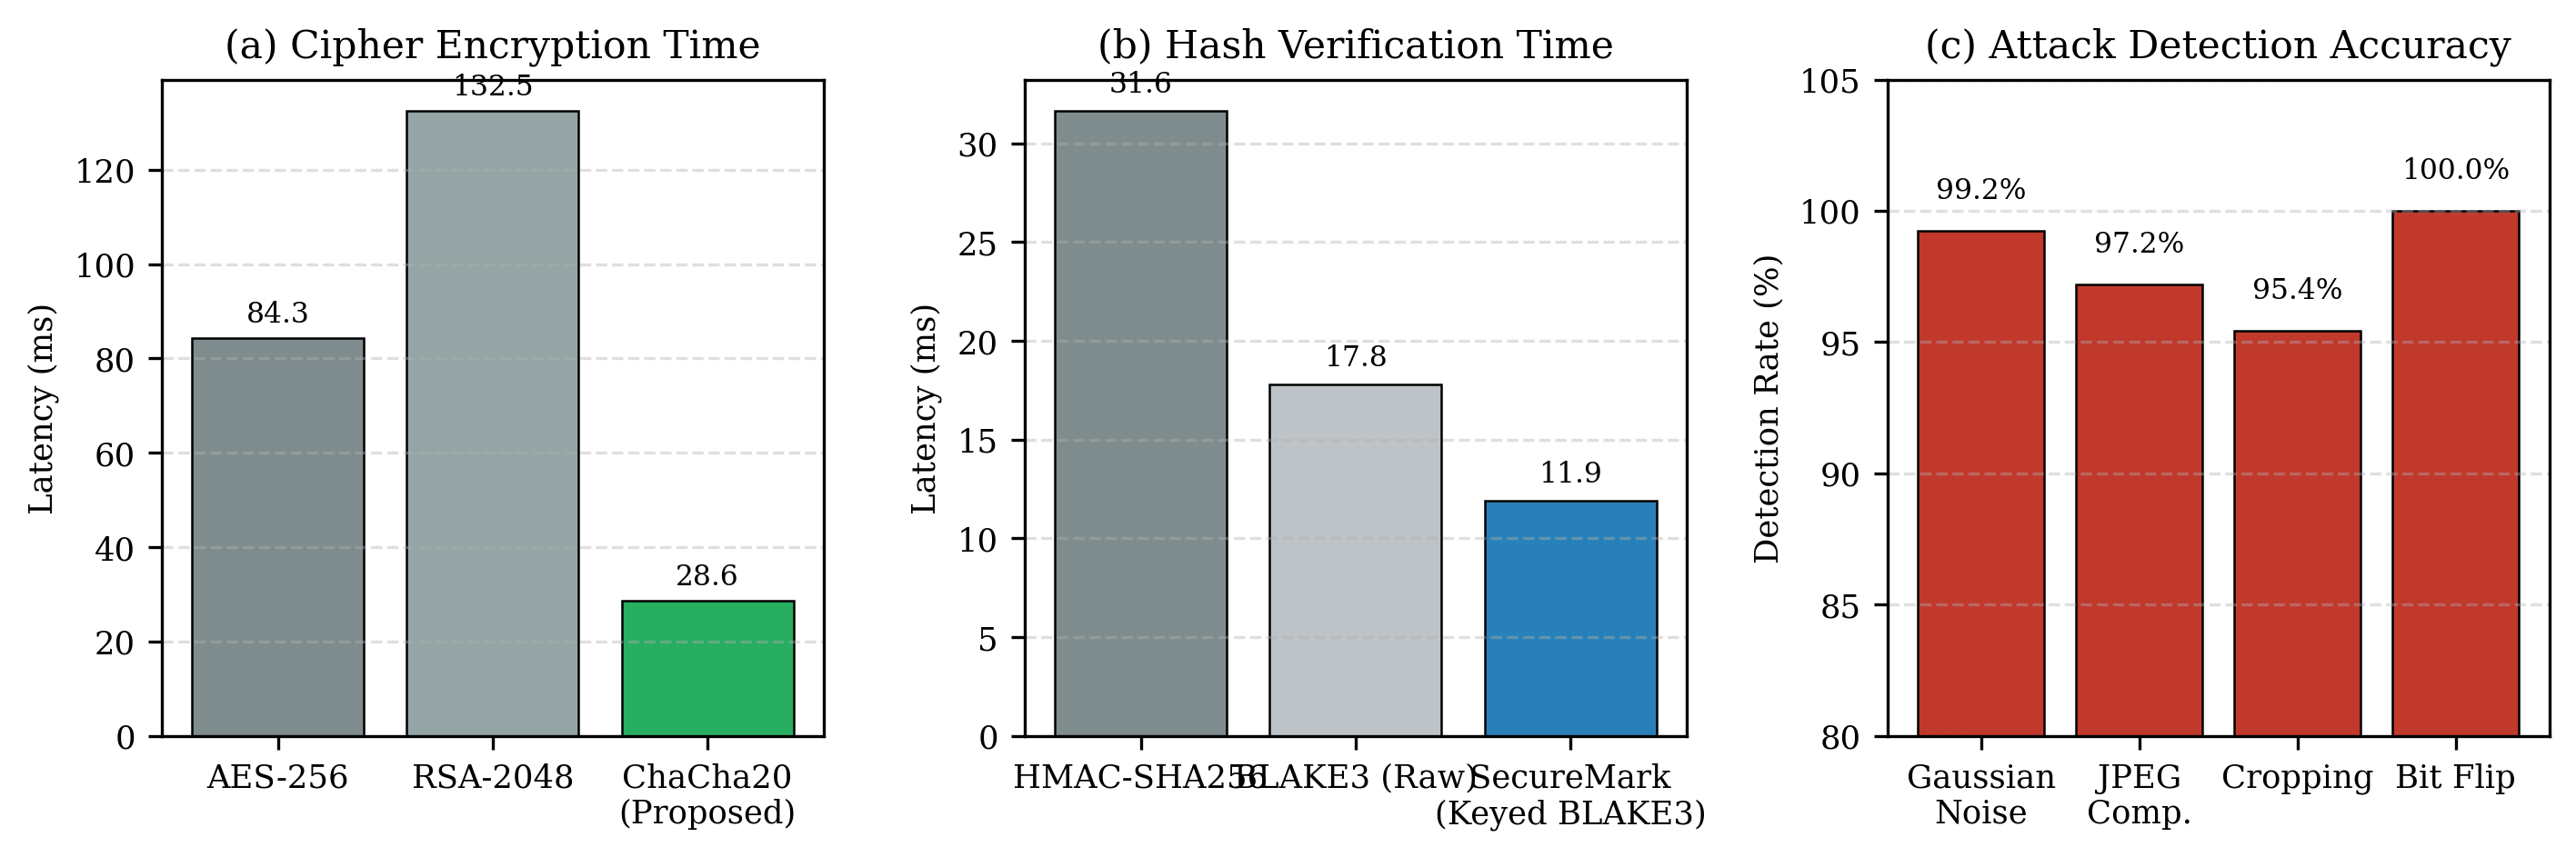
\includegraphics[width=0.8\textwidth]{fig_benchmarks.png}
\vspace{-5pt}
\caption{Performance benchmarks: (a) cipher encryption latency, (b) hash verification delay, and (c) attack detection accuracy across the evaluated vectors.}
\label{fig:benchmarks}
\end{figure}

\subsection{Diagnostic Image Fidelity}
Image fidelity was evaluated using Peak Signal-to-Noise Ratio (PSNR), Structural Similarity (SSIM), Normalized Cross-Correlation (NC), and Bit Error Rate (BER). PSNR was calculated from the mean-squared error between the original image $I$ and the watermarked image $I_w$:
\begin{equation}
  \text{PSNR} = 10\log_{10}\!\left(\frac{\text{MAX}_I^2}{\text{MSE}}\right), \quad
  \text{MSE} = \frac{1}{MN}\sum_{i=0}^{M-1}\sum_{j=0}^{N-1} \bigl[I(i,j)-I_w(i,j)\bigr]^2
\end{equation}

The visual comparison in Fig.~\ref{fig:visual_fidelity} is consistent with the numerical results in Table~\ref{tab:dataset_fidelity}. The original and watermarked chest X-ray appear nearly identical at normal viewing scale, while the amplified residual map makes the small LSB-level differences visible. For this sample, the measured PSNR is $52.14\,\text{dB}$ and SSIM is 0.9998.

\begin{figure}[t]
\centering
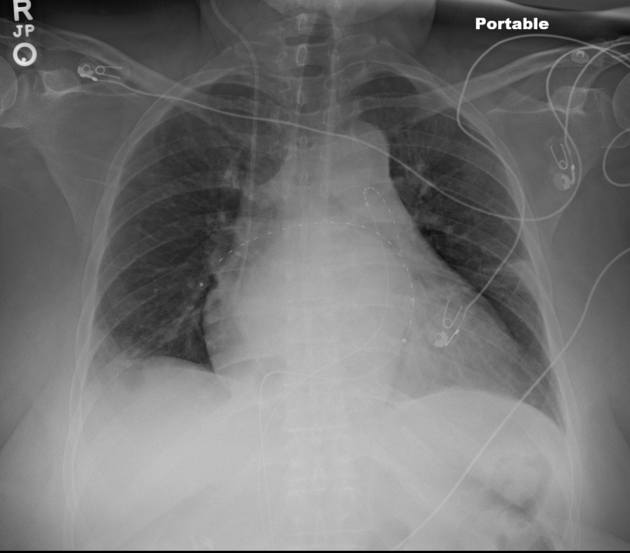
\includegraphics[width=0.8\textwidth]{fig_visual_fidelity.png}
\vspace{-5pt}
\caption{Chest X-ray example showing the original image, the watermarked image, and an amplified residual map. The reported sample has $\text{PSNR} = 52.14\,\text{dB}$ and $\text{SSIM} = 0.9998$.}
\label{fig:visual_fidelity}
\end{figure}

\subsection{5G Transmission Resilience and Tamper Detection}
A simulated 5G New Radio sub-6 GHz scenario was used to examine the deployment behavior shown in Fig.~\ref{fig:resilience}. End-to-end latency increased with payload size, but the SecureMark-Med curve remained below 1\,s for the tested payloads. In the intentional bit-flip tests, the verification chain detected all reported tampering attempts. The layers contribute different checks: AEAD identifies ciphertext changes, keyed BLAKE3 checks the authenticated recovered image, and the watermark comparison checks embedded provenance. Under non-adversarial degradations such as 5\% Gaussian noise and 50\% JPEG compression, the fragile watermark is expected to react to altered pixels; the reported detection rates were at least 95\% in the tested cases. This sensitivity is deliberate, although it also means that the current fragile watermark is intended for lossless or tightly controlled image paths rather than for routine lossy re-encoding.

\begin{figure}[t]
\centering
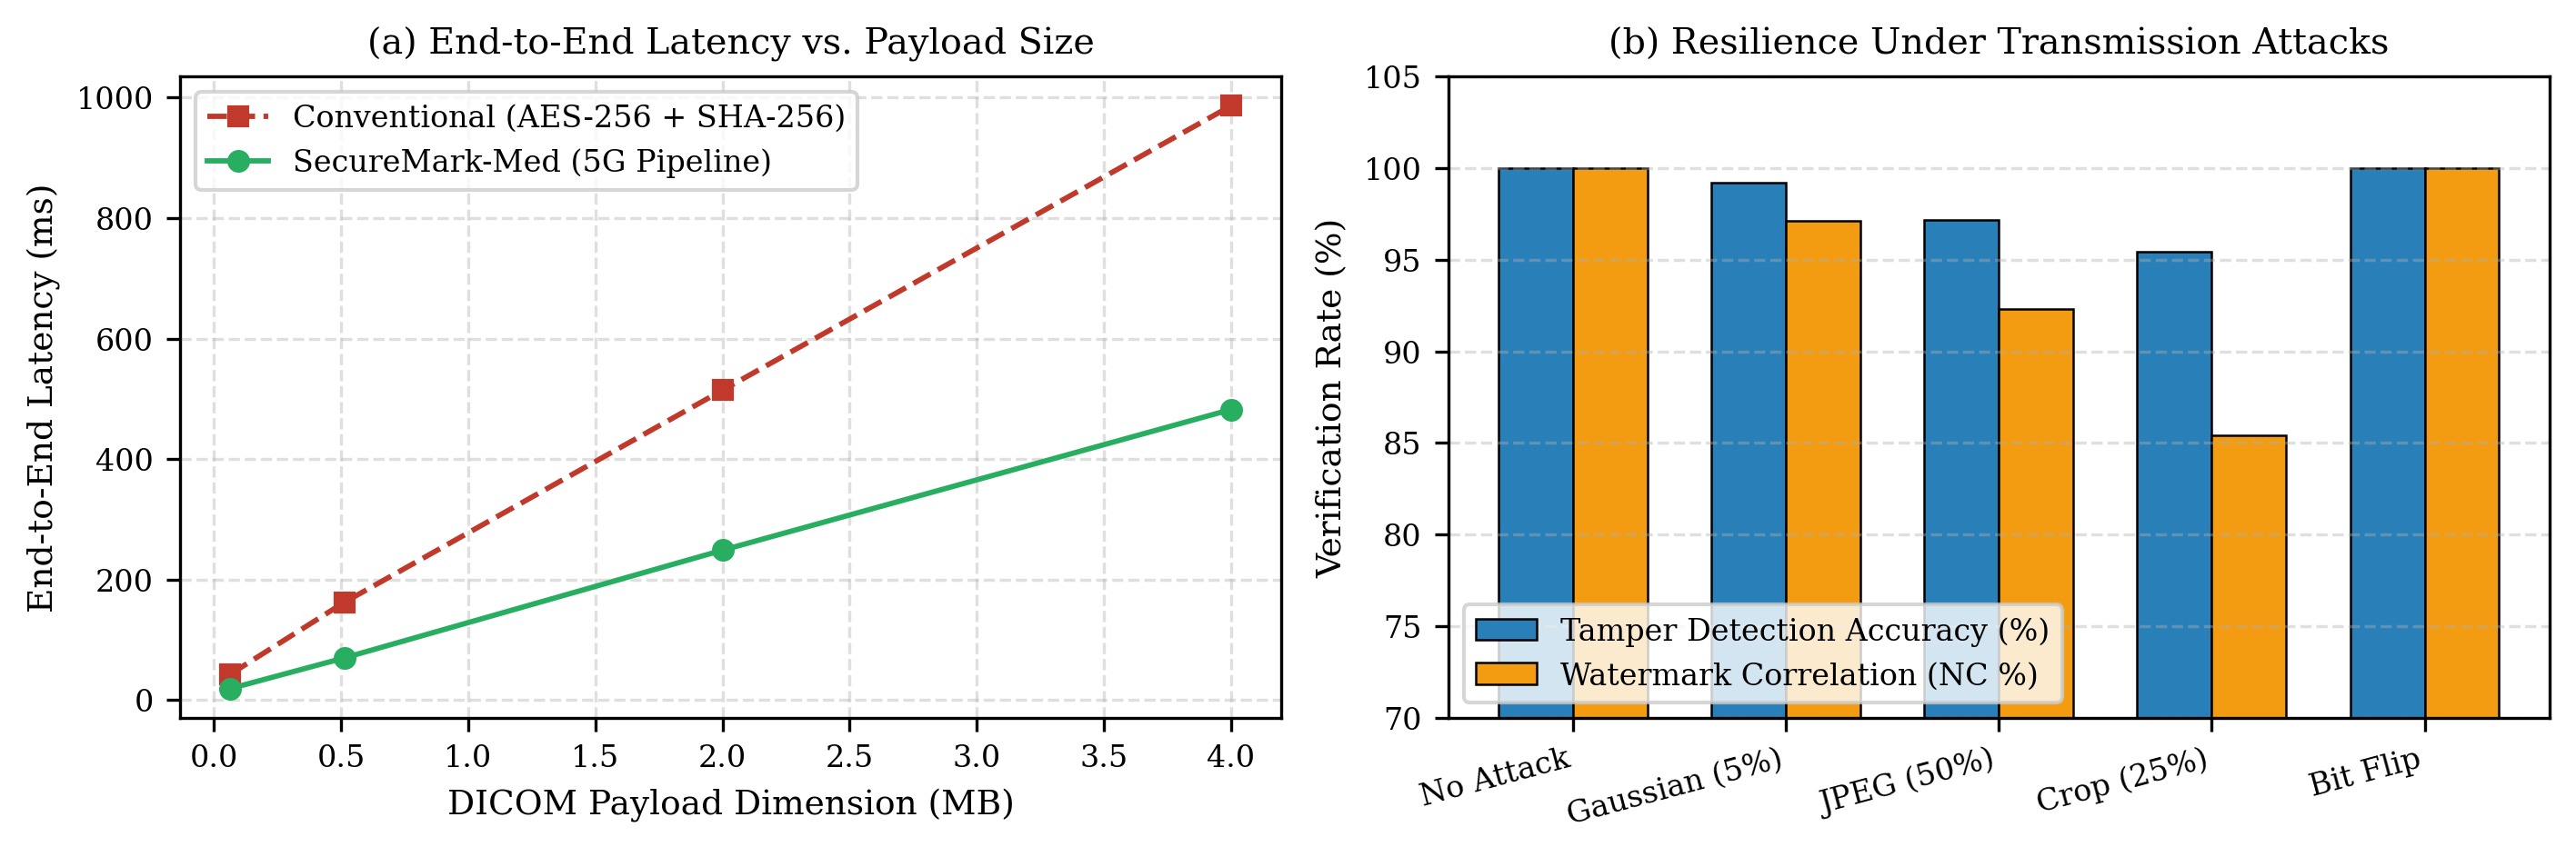
\includegraphics[width=0.8\textwidth]{fig_telemetry_resilience.png}
\vspace{-5pt}
\caption{5G telemetry performance and attack detection: (a) end-to-end latency versus payload size and (b) verification behavior under the evaluated transmission attacks.}
\label{fig:resilience}
\end{figure}

\section{Conclusion}
SecureMark-Med combines three complementary mechanisms for emergency DICOM telemetry: a fragile LSB watermark that keeps provenance information with the image, keyed BLAKE3 for application-layer integrity binding, and ChaCha20-Poly1305 for authenticated transport. On the Raspberry Pi 3 Model B+ test platform, the proposed cryptographic stages required $28.61\,\text{ms}$ for encryption and $11.92\,\text{ms}$ for verification, compared with $84.32\,\text{ms}$ and $31.65\,\text{ms}$ for the reported AES-256 and HMAC-SHA256 baselines. The tested images also retained high fidelity, with the 16-bit cases exceeding $51.4\,\text{dB}$ PSNR and 0.999 SSIM, while the listed BER remained 0.00\%. These results support the feasibility of the design for edge telemetry under the evaluated conditions. A limitation of the present fragile watermark is its sensitivity to lossy processing. Future work will therefore investigate automated region-of-interest segmentation and strategies that preserve diagnostic regions when transmission or storage involves controlled lossy operations.

\begin{thebibliography}{14}
\small
\setlength{\itemsep}{0pt}
\setlength{\parskip}{0pt}
\setlength{\parsep}{0pt}

\bibitem{memon2020prediction}
Memon, N.A., Alzahrani, A.: Prediction-based reversible watermarking of CT
scan images for content authentication and copyright protection. IEEE Access \textbf{8},
75448--75462 (2020). \doi{10.1109/ACCESS.2020.2989175}

\bibitem{anand2021health}
Anand, A., Singh, A.K.: Health record security through multiple watermarking
on fused medical images. IEEE Trans. Comput. Soc. Syst. \textbf{9}(6), 1594--1603 (2021).
\doi{10.1109/TCSS.2021.3126628}

\bibitem{alzahrani2021blind}
Alzahrani, A., Memon, N.A.: Blind and robust watermarking scheme in hybrid
domain for copyright protection of medical images. IEEE Access \textbf{9}, 113714--113734
(2021). \doi{10.1109/ACCESS.2021.3104985}

\bibitem{gull2021self}
Gull, S., Mansour, R.F., Aljehane, N.O., Parah, S.A.: A self-embedding
technique for tamper detection and localization of medical images for smart-health.
Multimed. Tools Appl. \textbf{80}(19), 29939--29964 (2021). \doi{10.1007/s11042-021-11170-x}

\bibitem{singh2023robust}
Singh, P., Devi, K.J., Thakkar, H.K., Bilal, M., Nayyar, A., Kwak, D.: Robust and
secure medical image watermarking for edge-enabled e-healthcare. IEEE Access \textbf{11},
135831--135845 (2023). \doi{10.1109/ACCESS.2023.3335172}

\bibitem{tayachi2023hybrid}
Tayachi, M., Nana, L., Pascu, A.C., Benzarti, F.: A hybrid watermarking approach
for DICOM images security. Appl. Sci. \textbf{13}(10), 6132 (2023). \doi{10.3390/app13106132}

\bibitem{abirami2024secured}
Abirami, R., Malathy, C.: Secured DICOM medical image transition with optimized
chaos method for encryption and customized deep learning model for watermarking.
Automatika \textbf{66}(2) (2025). \doi{10.1080/00051144.2025.2460877}

\bibitem{mahmood2025secure}
Mahmood, S.D., Drira, F., Mahdi, H.F., Alimi, A.M.: Secure medical image sharing:
Technologies, watermarking insights, and open issues. IEEE Access \textbf{13},
103995--104026 (2025). \doi{10.1109/ACCESS.2025.3574477}

\bibitem{singh2025ensuring}
Singh, P., Devi, K.J., Nayyar, A., Bilal, M.: Ensuring integrity and security of
medical image transmission in IoMT applications through robust watermarking.
Sci. Rep. \textbf{15}(1), 14210 (2025). \doi{10.1038/s41598-025-11023-9}

\bibitem{jasim2025optimizing}
Jasim, Z.A., Hadi, A.K.: Optimizing blockchain network performance using BLAKE3
hash function in POS consensus algorithm. IEEE Access \textbf{13}, 44760--44774 (2025).
\doi{10.1109/ACCESS.2025.3546723}

\bibitem{buhler2022benchmarking}
Bühler, H., Walz, A., Sikora, A.: Benchmarking of Symmetric Cryptographic
Algorithms on a Deeply Embedded System. IFAC-PapersOnLine \textbf{55}(4),
266--271 (2022). \doi{10.1016/j.ifacol.2022.06.044}

\bibitem{oconnor2020blake3}
O'Connor, J., Aumasson, J.P., Neves, S., Wilcox-O'Hearn, Z.: BLAKE3: One
function, fast everywhere. Real World Crypto (2020). \doi{10.5281/zenodo.3899478}

\bibitem{nir2018chacha20}
Nir, Y., Langley, A.: ChaCha20 and Poly1305 for IETF Protocols. RFC 8439,
Internet Engineering Task Force (2018). \doi{10.17487/RFC8439}

\bibitem{nema2024dicom}
NEMA: Digital Imaging and Communications in Medicine (DICOM) Standard,
PS3.1--PS3.20. National Electrical Manufacturers Association, Rosslyn, VA (2024).
Available at: \url{https://www.dicomstandard.org/}

\end{thebibliography}

\end{document}